\documentclass{article}
\usepackage{graphicx} % Required for inserting images
\usepackage{amsmath}
\usepackage{tikz}
\usetikzlibrary{shapes.geometric, arrows}
\usepackage{hyperref}
\usepackage{float}
\usepackage{caption}
%%%%%%%%%%%%%%%%%%%%%%%%%%%%%%%%%%%%%%%%%%%%%%%%%%%%
\tikzstyle{startstop} = [rectangle, rounded corners, minimum width=3cm, minimum height=1cm,text centered, draw=black, thick]
\tikzstyle{process} = [rectangle, minimum width=3cm, minimum height=1cm, text centered, draw=black, thick]
\tikzstyle{decision} = [diamond, minimum width=1cm, minimum height=1cm, text centered, draw=yellow, thick]
\tikzstyle{arrow} = [thick,->,>=stealth,draw=green]
\tikzstyle{arrowloop} = [thick,->,>=stealth, draw=blue]
%%%%%%%%%%%%%%%%%%%%%%%%%%%%%%%%%%%%%%%%%%%%%%%%%%%%%

\title{Elaboração e representação gráfica dos vetores campo elétrico e campo magnético de uma carga pontual com velocidade constante não relativística considerando a velocidade de propagação do campo utilizando Fortran e Python }
\author{Murilo Garcia e Maria Eduarda}
\date{Janeiro 2025}


\begin{document}
\maketitle
\newpage
\section{Introdução}
\hspace{0.45cm}O projeto em questão consiste da elaboração de um programa que calcule em determinados pontos do espaço os vetores produzidos por uma carga elétrica em movimento para certos instantes de tempo em um dado período. Após isso realiza-se o plot dos vetores para demonstrar visualmente como se dá a dinâmica eletromagnética.

\section{Contextualização teórica}
\hspace{0.45cm}Pela teoria eletromagnética clássica cargas elétricas em movimento relativo a um dado referencial geram campos magnéticos, tais campos são descritos  pelas equações de Maxwell abaixo. Em especial nos interessa mais Lei de Ampére-Maxwell.


\begin{align}
    \nabla \cdot \vec{\mathbf{E}} &= \frac{\rho}{\epsilon_0} \quad &\text{(Lei de Gauss para o campo elétrico)} \\
    \nabla \cdot \vec{\mathbf{B}} &= 0 \quad &\text{(Lei de Gauss para o campo magnético)} \\
    \nabla \times \vec{\mathbf{E}} &= -\frac{\partial \vec{\mathbf{B}}}{\partial t} \quad &\text{(Lei de Faraday)} \\
    \nabla \times \vec{\mathbf{B}} &= \mu_0 \vec{\mathbf{J}} + \mu_0 \epsilon_0 \frac{\partial \vec{\mathbf{E}}}{\partial t} \quad &\text{(Lei de Ampère-Maxwell)}
\end{align}

\vspace{0.3cm}


Assim, através de manipulações envolvendo Teorema de Helmholtz \textbf{(colocar referência)} e Lei de Biot-Savart conseguimos manipular a expressão para o campo magnético e para o campo elétrico. De maneira sucinta vamos trabalhar primeiramente com o campo elétrico $\vec{\mathbf{E}}$.

\subsection{Campo Elétrico $\vec{\mathbf{E}}$}

\hspace{0.45cm}Dado um vetor $\vec{\mathbf{R}}(x,y,z)$ que denota qualquer posição no espaço e um vetor $\vec{\mathbf{r}}(x,y,z)$ que denota a posição da carga no espaço podemos escrever o Potencial Elétrico gerado por essa carga como:
\begin{equation}
    V(\vec{\mathbf{R}}) = \frac{q}{|\vec{\mathbf{R}} - \vec{\mathbf{r}}|}
\end{equation}
\hspace{0.45cm}Logo
\begin{equation}
    \vec{\mathbf{E}}(\vec{\mathbf{R}}) = - \frac{\partial V}{\partial \vec{\textbf{R}}}
\end{equation}
\hspace{0.45cm}Considerando que o campo se propaga no espaço com velocidade constante igual a \textbf{c} há um certo instante de tempo mesmo que pequeno para que este alcance tal ponto do espaço de modo que há uma "retardação" do campo nesses pontos. Para levarmos esse fato em consideração devemos calcular esta diferença de tempo entre o tempo próprio da carga simbolizado por $\mathbf{t}$ e o tempo retardado no qual chamaremos de $\mathbf{t_{ret}}$. Utilizando princípios básicos de cinemática encontramos:
\begin{equation}
    \mathbf{t_{ret}} = \mathbf{t} - \frac{|\vec{\mathbf{R}} - \vec{\mathbf{r}}\mathbf{(t_{ret})}|}{c}
\end{equation}
\hspace{0.45cm}O que nos leva a seguinte equação para o Potencial Elétrico:
    

\begin{equation}
    V(\mathbf{R} , \mathbf{t}) = \frac{q}{|\vec{\mathbf{r}}_\mathbf{ret}|(1 - \hat{\mathbf{r}}_\mathbf{ret} \cdot \frac{\vec{\mathbf{v}}_\mathbf{ret}}{c}) } 
\end{equation}

No qual o vetor $\vec{\mathbf{v}}_\mathbf{ret}$ corresponde ao vetor velocidade da partícula calculada no instante $\mathbf{t} = \mathbf{t_{ret}}$, de maneira análoga o vetor $\vec{\mathbf{r}}_\mathbf{ret}$ está para o vetor posição da partícula no instante $\mathbf{t_{ret}}$. Agora precisamos adicionar o termo responsável pelo campo magnético de modo que pelo Teorema de Helmholtz juntamente ao potencial vetor $\vec{\mathbf{A}}$ para o campo magnético obtemos:

\begin{equation}
    \vec{\mathbf{E}} = -\vec{\mathbf{\nabla}}V - \frac{1}{c}\frac{\partial \vec{\mathbf{A}}}{\partial t}
\end{equation}
\hspace{0.45cm}Se definirmos o potencial vetor como simplesmente $\vec{\mathbf{A}} = \frac{q \vec{\mathbf{v}}}{|\vec{\mathbf{R}} - \vec{\mathbf{r}}|c}$ chegamos na expressão final para o campo elétrico dependente do tempo:
\begin{equation}
    \vec{\mathbf{E}}(\vec{\mathbf{R}}, \mathbf{t}) = \frac{q|\vec{\mathbf{r}}_{ret}|}{(\vec{\mathbf{r}}_\mathbf{ret} \cdot \vec{\mathbf{u}}_\mathbf{ret})^3}[\vec{\mathbf{u}}_\mathbf{ret}(c^2 - |\vec{\mathbf{v}}_\mathbf{ret}|^2) + \vec{\mathbf{r}}_\mathbf{ret} \times (\vec{\mathbf{u}}_\mathbf{ret} \times \vec{\mathbf{a}}_\mathbf{ret})]
\end{equation}
\begin{center}
    Onde $\vec{\mathbf{u}}_\mathbf{ret} \equiv c\hat{\mathbf{r}}_\mathbf{ret} - \vec{\mathbf{v}}_\mathbf{ret}$
\end{center}
Apesar do termo $\vec{\mathbf{R}}$ não estar de forma explícita na equação acimam assim como $\mathbf{t_{ret}}$ todos os termos com subíndice \textbf{ret} estão sendo calculados através de $\mathbf{t_{ret}}$ que por sua vez é calculado dado um vetor posição $\vec{\mathbf{R}}$.
\subsection{Campo Magnético $\vec{\mathbf{B}}$}
\hspace{0.45cm}O campo magnético pode ser obtido através do vetor potencial sobe a igualdade $\mathbf{\nabla} \times \vec{\mathbf{A}} = \vec{\mathbf{B}}$ mas podemos verificar facilmente que:
\begin{equation}
    \vec{\mathbf{B}} = \hat{\mathbf{r}}_\mathbf{ret} \times \vec{\mathbf{E}}
\end{equation}
\newpage
\vspace{-1cm}
\section{Etapa Computacional}
\hspace{0.45cm} A etapa computacional pode ser resumida no seguinte fluxograma:
\begin{center}
    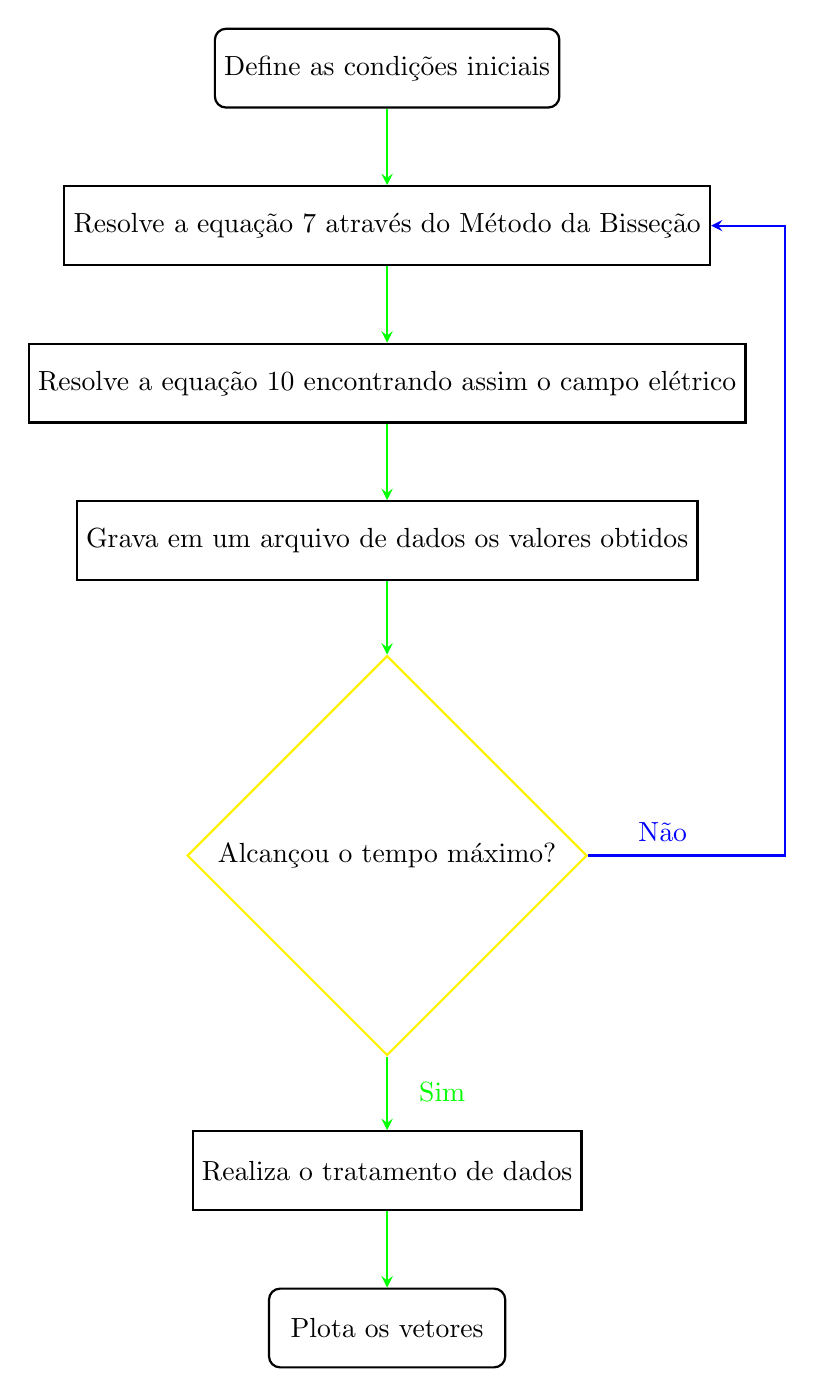
\begin{tikzpicture}[node distance=2cm]

        % Nós (blocos do fluxograma)
        \node (start) [startstop] {Define as condições iniciais};
        \node (process1) [process, below of=start] {Resolve a equação 7 através do Método da Bisseção};
        \node (process2) [process, below of=process1] {Resolve a equação 10 encontrando assim o campo elétrico};
        \node (process3) [process, below of=process2] {Grava em um arquivo de dados os valores obtidos};
        \node (decision) [decision, below of=process3, node distance=4cm] {Alcançou o tempo máximo?};
        \node (process4) [process, below of=decision, node distance=4cm] {Realiza o tratamento de dados};
        \node (process5) [startstop, below of=process4] {Plota os vetores};

        % Conexões entre os nós (setas)
        \draw [arrow] (start) -- (process1);
        \draw [arrow] (process1) -- (process2);
        \draw [arrow] (process2) -- (process3);
        \draw [arrow] (process3) -- (decision);
        \draw [arrow] (decision) -- (process4);
        \draw [arrow] (process4) -- (process5);

        % Loop de repetição caso não tenha alcançado o tempo máximo
        \node (textno) [right of=decision, xshift=1.5cm, yshift = 0.3cm] {\textcolor{blue}{Não}};
        \draw [arrowloop] (decision.east) -- ++(2.5,0) |- (process1.east);
        \node(textno) [above of=process4, xshift=0.7cm,yshift=-1cm]{\textcolor{green}{Sim}};

    \end{tikzpicture}
\end{center}
\begin{center}
    \textbf{Fluxograma 1}
\end{center}
\hspace{0.45cm}De todas as etapas no Fluxograma 1 apenas as duas últimas foram realizadas utilizando a linguagem Python enquanto as outras utilizando Fortran90. Isto é, a etapa de cálculos e de inúmeros loops necessários foi-se utilizado Fortran já enquanto para parte gráfica e tratamento de dados, Python. 
\subsection{Adaptações e Dificuldades}
\hspace{0.45cm}Conforme o estudo da teoria, os limites de conhecimento dos integrantes do grupo e pelo tempo optou-se por simplificar a situação física e também matemática. Segue algumas medidas mais importantes:
\begin{itemize}
    \item[1$\xrightarrow{}$] Tomamos o caso em que a velocidade da partícula é constante no tempo o que implica que sua aceleração é nula. Portanto, não há emissão de radiação eletromagnética por parte da partícula e com isso a equação 10 se torna:
\end{itemize}

\begin{equation}
    \vec{\mathbf{E}}(\vec{\mathbf{R}}, \mathbf{t}) = \frac{q|\vec{\mathbf{r}}_{ret}|}{(\vec{\mathbf{r}}_\mathbf{ret} \cdot \vec{\mathbf{u}}_\mathbf{ret})^3}\vec{\mathbf{u}}_\mathbf{ret}(c^2 - |\vec{\mathbf{v}}_\mathbf{ret}|^2)
\end{equation}
\begin{itemize}
    \item[2$\xrightarrow{}$] Outra complicação surge da resolução da equação 7 que pode vir a ser muito complicada a depender da trajetória do objeto, ao nosso caso, mais simples com velocidade constante a equação vem a ser:
    \begin{equation}
        \mathbf{t_{ret}} = \mathbf{t} - \frac{\sqrt{(X-V_{x}\mathbf{t_{ret}})^2 + (Y-V_y\mathbf{t_{ret})}^2 + (Z-V_z\mathbf{t_{ret}}})^2}{c}
    \end{equation}
    Nessa representação as tripla \textbf{(X,Y,Z)} e $\mathbf{(V_{x}, V_{y}, V_{z})}$ correspondem as coordenadas dos vetores posição $\vec{\mathbf{R}}$ e velocidade $\vec{\mathbf{v}}$ respectivamente.
    A solução é extremamante complicada, porém possível. Difícil averiguar também para quais valores reais essa equação assume solução em  $\mathbf{t_{ret}}$. Seguindo a referência principal dos estudos para esse trabalho e após algumas conversas com o professor decidimos utilizar o Método da Bisseção para encontrar valores aproximados das soluções dessa equação.
    \item[3$\xrightarrow{}$] Devido ao fato da variável  ser do tipo  mesmo para o instante de tempo  ela variava consideravelmente sendo necessário tomar uma média desses valores e o adotando como respectivos novos valores para o plot.
    \item[4$\xrightarrow{}$] Por último mas não menos importante foi perceptível ao analisar o arquivo de dados gerado que o campo elétrico $\vec{\mathbf{E}}$ pouco variava para os valores das coordenadas X,Y,Z escolhidas sendo necessária modificação desses pontos para cada vez mais próximos da partícula. Uma tentativa alternativa foi aumentar o valor da carga mas não hove mudanças significativas.
\end{itemize}
\subsection{O Programa}
O programa é consistido de três arquivos:
\begin{itemize}
    \item[\textbf{Arquivo 1} $\xrightarrow{}$] \textbf{cargas\_modulo.f90 :}
    O arquivo é um módulo obrigatório que consiste de todas as funções, objetos e subrotinas necessárias para a execução do programa. Sem ele nada irá funcionar. Ele possui:
    \begin{itemize}
        \item[\textbf{a)}] Objeto carga dotado de caracaterísitca como posição inicial e velocidade.
        \item[\textbf{b)}] Funções:
        \begin{itemize}
            \item trajetória: Calcula onde a partícula está para cada instante de tempo \textbf{t} ou seja, o vetor $\vec{\textbf{r}}$.
            \item calcula\_modulo: Responsável por retornar o módulo de qualquer vetor em n dimensões no espaço euclidiano.
            \item normaliza\_vetor: Normaliza o vetor e o retorna normalizado.
            \item g: Função que gera a equação 7.
            \item solve: Método da Bisseção retornando a solução aproximada da equação feita na função \textbf{g}.   
        \end{itemize}
        \item[\textbf{c)}] Uma única subrotina chamada escreve\_dados que há alguns problemas e acabou não sendo utilizada mas presente para futura implementação e melhoria.
    \end{itemize}
    \item[\textbf{Arquivo 2 $\xrightarrow{}$}] \textbf{programa.f90:} Este é o programa principal onde o usuário deverá inserir as condições físicas iniciais do problema: velocidade e posição inicial além de também poder alterar o número de imagens geradas e tempo de simulação, logo controlar o FPS. A descrição de como realizar se encontra no arquivo \textbf{readme.md} disponível em \href{https://github.com/Kiberan/Projeto_Final_Fis492}{Repositório}.
    \item[\textbf{Arquivo 3 $\xrightarrow{}$}] \textbf{plot.py:} Responsável pelo tratamento de dados conforme dito anteriormente e também pela parte visual/gráfica. Se encontra atualmente incompleto em andamento.
\end{itemize}
\newpage
\subsection{Conclusão}
De todo trabalho realizado até aqui atualmente apenas a etapa de criação dos dados é a mais próxima de estar completa e em perfeitas condições a menos de alguns erros e situações conformes ditas anteriormente. Segue uma imagem de um trecho de um arquivo.dat gerado em testes:
\begin{figure}[H]
    \centering
    \includegraphics[width=1\linewidth]{Print dos dados.png}
    \captionsetup{labelformat=empty}
    \caption{Captura de tela de um arquivo.dat gerado em um dos testes}
    \label{fig:enter-label}
\end{figure}
Na imagem acima fica claramente o problema de float com tempo negativo sendo que correspondem a \textbf{t = 0}.
Infelizmente o projeto não pode ser concluído mas fica o imenso aprendizado e resolução de inúmeros problemas que não puderam ser descritos aqui pela falta de tempo providas principalmente de situações pessoais de indivíduos do grupo.
\subsection{Referências Bibliográficas}
\begin{itemize}
    \item [1] An Introduction to Computer Simulation Methods Applications to Physical System .Harvey Gould, Jan Tobochnik, and Wolfgang Christian. Disponível em \href{https://www.compadre.org/osp/items/detail.cfm?ID=7375}{Compadre}.
    \item [2] Notas de Aula do Professor Wesley Cota. Disponível em \href{https://fis492.wcota.me/}{Notas de Aula}
\end{itemize}
Fica aqui nosso imenso agradecimento ao professor Wesley pela paciência e dedicação com todas as intempéries ocorridas ao longo desse semestre e sua imensa abertura para nos ajudar. Isso ajuda muito e dá forças para concluir o curso e seguir em frente. Obrigado!
\end{document}
